\documentclass{beamer}
\mode<presentation>{
	\usetheme{Madrid}
}
\usepackage{graphicx}
\usepackage{listings}
\graphicspath{{./img}}
\usepackage[backend=bibtex, sorting=none]{biblatex}
\addbibresource{./bib/bib.bib}
\usepackage{polski}
\title[]{Rozpoznawanie liter języka migowego z zastosowaniem technik uczenia maszynowego}
\institute[UMCS]
{
	Uniwersytet Marii Curie Skłodowskiej
	\medskip
}
\author{Rafał Hrabia}
\date{\today}

\begin{document}
	% 1
	\begin{frame}
		\titlepage
	\end{frame}
	% 2
	\begin{frame}
		\frametitle{Cel pracy}
		\section{Cel pracy}
		\begin{itemize}
			\item Przybliżenie zagadnienia języka migowego American Sign Language oraz sieci konwolucyjnych CNN
			\item Stworzenie zbioru danych zawierających obrazy, na których znajdują się znaki języka migowego American Sign Language
			\item Stworzenie oraz wytrenowanie modelu rozpoznającego znaki języka migowego
			\item Implementacja programu (PoC) umożliwiającego rozpoznawanie języka migowego w czasie rzeczywistym
		\end{itemize}
	\end{frame}

	% 3
	\begin{frame}
		\frametitle{Istota pracy}
		\section{Istota pracy}
		\begin{itemize}
			\item Możliwe w przyszłości ułatwienie komunikacji osób nie znających języka migowego z osobami głuchoniemymi
		\end{itemize}
	\end{frame}

	% 4
	\begin{frame}
		\frametitle{Język migowy American Sign Language}
		\section{Język migowy American Sign Language}
		Jest to wariant języka migowego używanego w krajach obu Ameryk, gdzie natywnym językiem jest angielski.\cite{padden}
		
		Posiada 26 znaków (American manual alphabet), używanych do wyrażania słów.\cite{costello}
		
		Składnia języka opiera się na subject–verb–object (SVO) czyli w zdaniu występuje podmiot, orzeczenie i obiekt, do którego skierowany jest czasownik.\cite{neidle} Przykładowo:
		\begin{center}
			FATHER LOVE CHILD
			
			co będzie oznaczało
			
			"The father loves the child."
		\end{center}
	\end{frame}

	% 5
	\begin{frame}
		\frametitle{Język migowy American Sign Language}
		\section{Język migowy American Sign Language}
		\begin{center}
			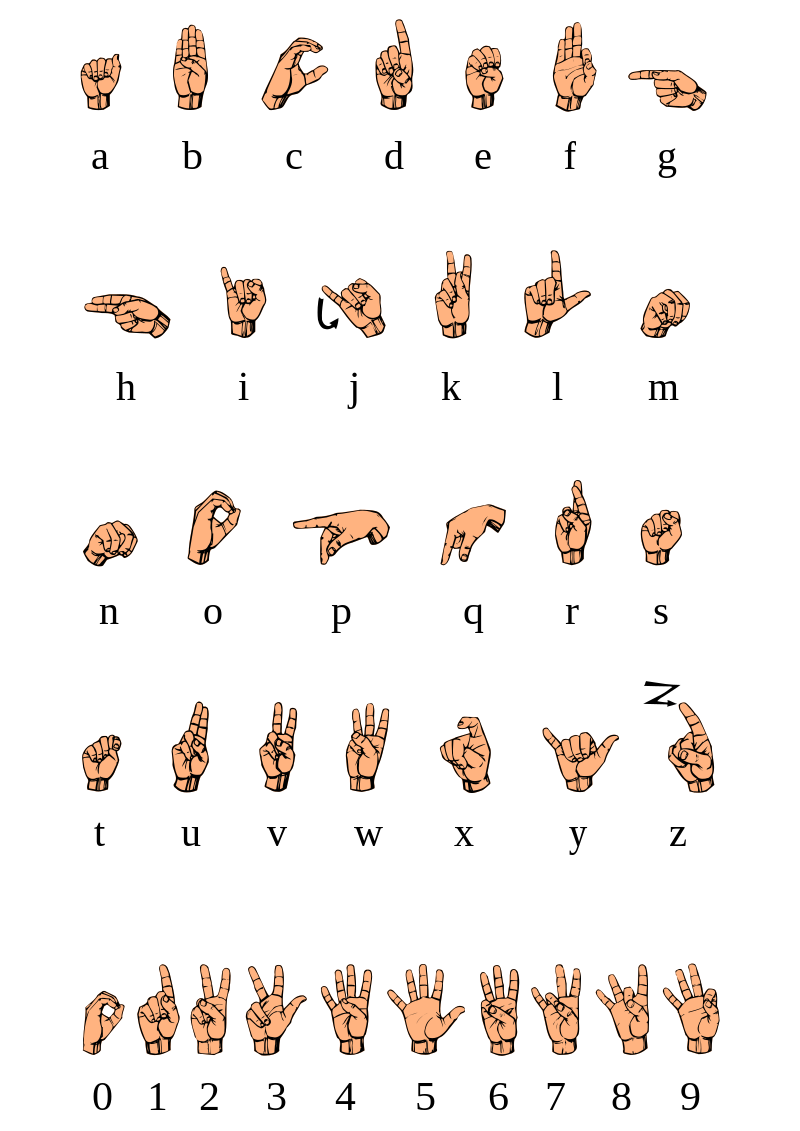
\includegraphics[scale=0.25]{Asl}
		\end{center}
	\end{frame}

	% 6
	\begin{frame}
		\frametitle{Treningowy zbiór danych}
		\section{Treningowy zbiór danych}
		Treningowy zbiór danych zawiera około 50 000 autorskich obrazów poszczególnych liter alfabetu ASL.
		\begin{center}
			\begin{tabular}{c|c|c|c}
				Litera & A & B & F \\
				\hline
				Obraz &
				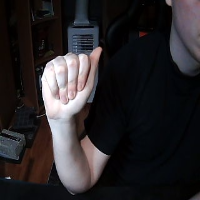
\includegraphics[scale=0.4]{1} &
				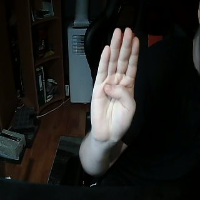
\includegraphics[scale=0.4]{2} &
				
\includegraphics[scale=0.4]{3}
			\end{tabular}
			
		\end{center}
	\end{frame}

	% 7
	\begin{frame}
		\frametitle{Model i architektura}
		\section{Model i architektura}
		\begin{center}
			\lstinputlisting[basicstyle=\linespread{0.1}\tiny]{model.txt}
		\end{center}
	\end{frame}

	% 8
	\begin{frame}
		\frametitle{Trening modelu}
		\section{Model i architektura}
		Model osiąga przyzwoite wyniki rzędu 85-90\% dokładności klasyfikacji na zbiorze walidacyjnym.
		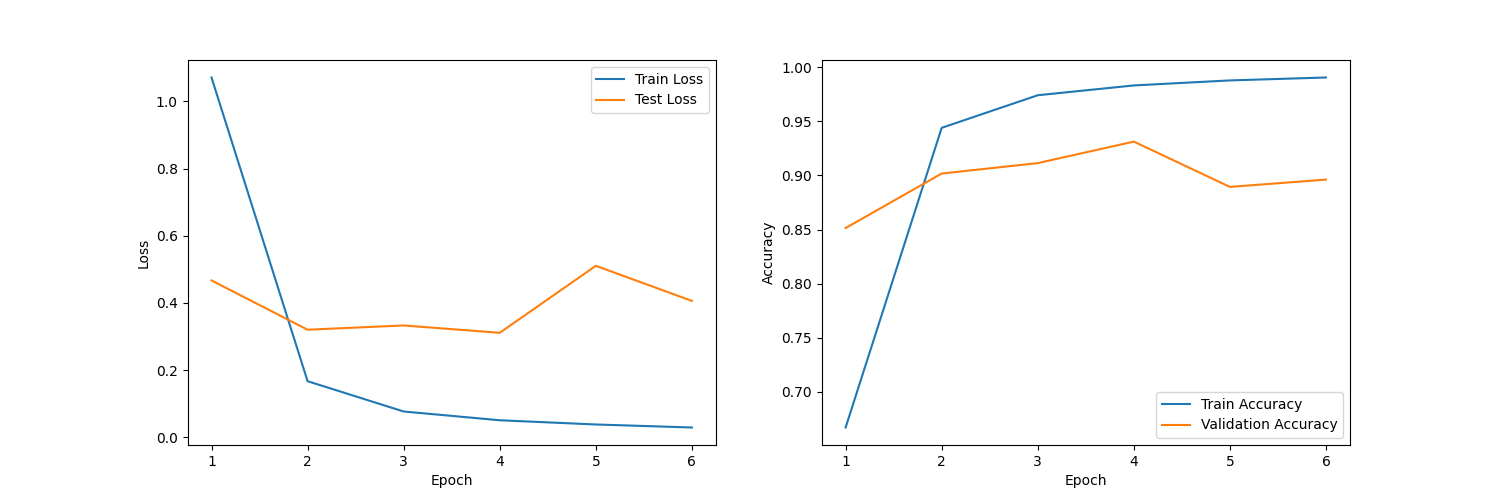
\includegraphics[scale=0.23]{myplot}
	\end{frame}

	% 9
	\begin{frame}
		\frametitle{Program do rozpoznawania języka migowego w czasie rzeczywistym}
		\section{Program do rozpoznawania języka migowego w czasie rzeczywistym}
		\begin{center}
			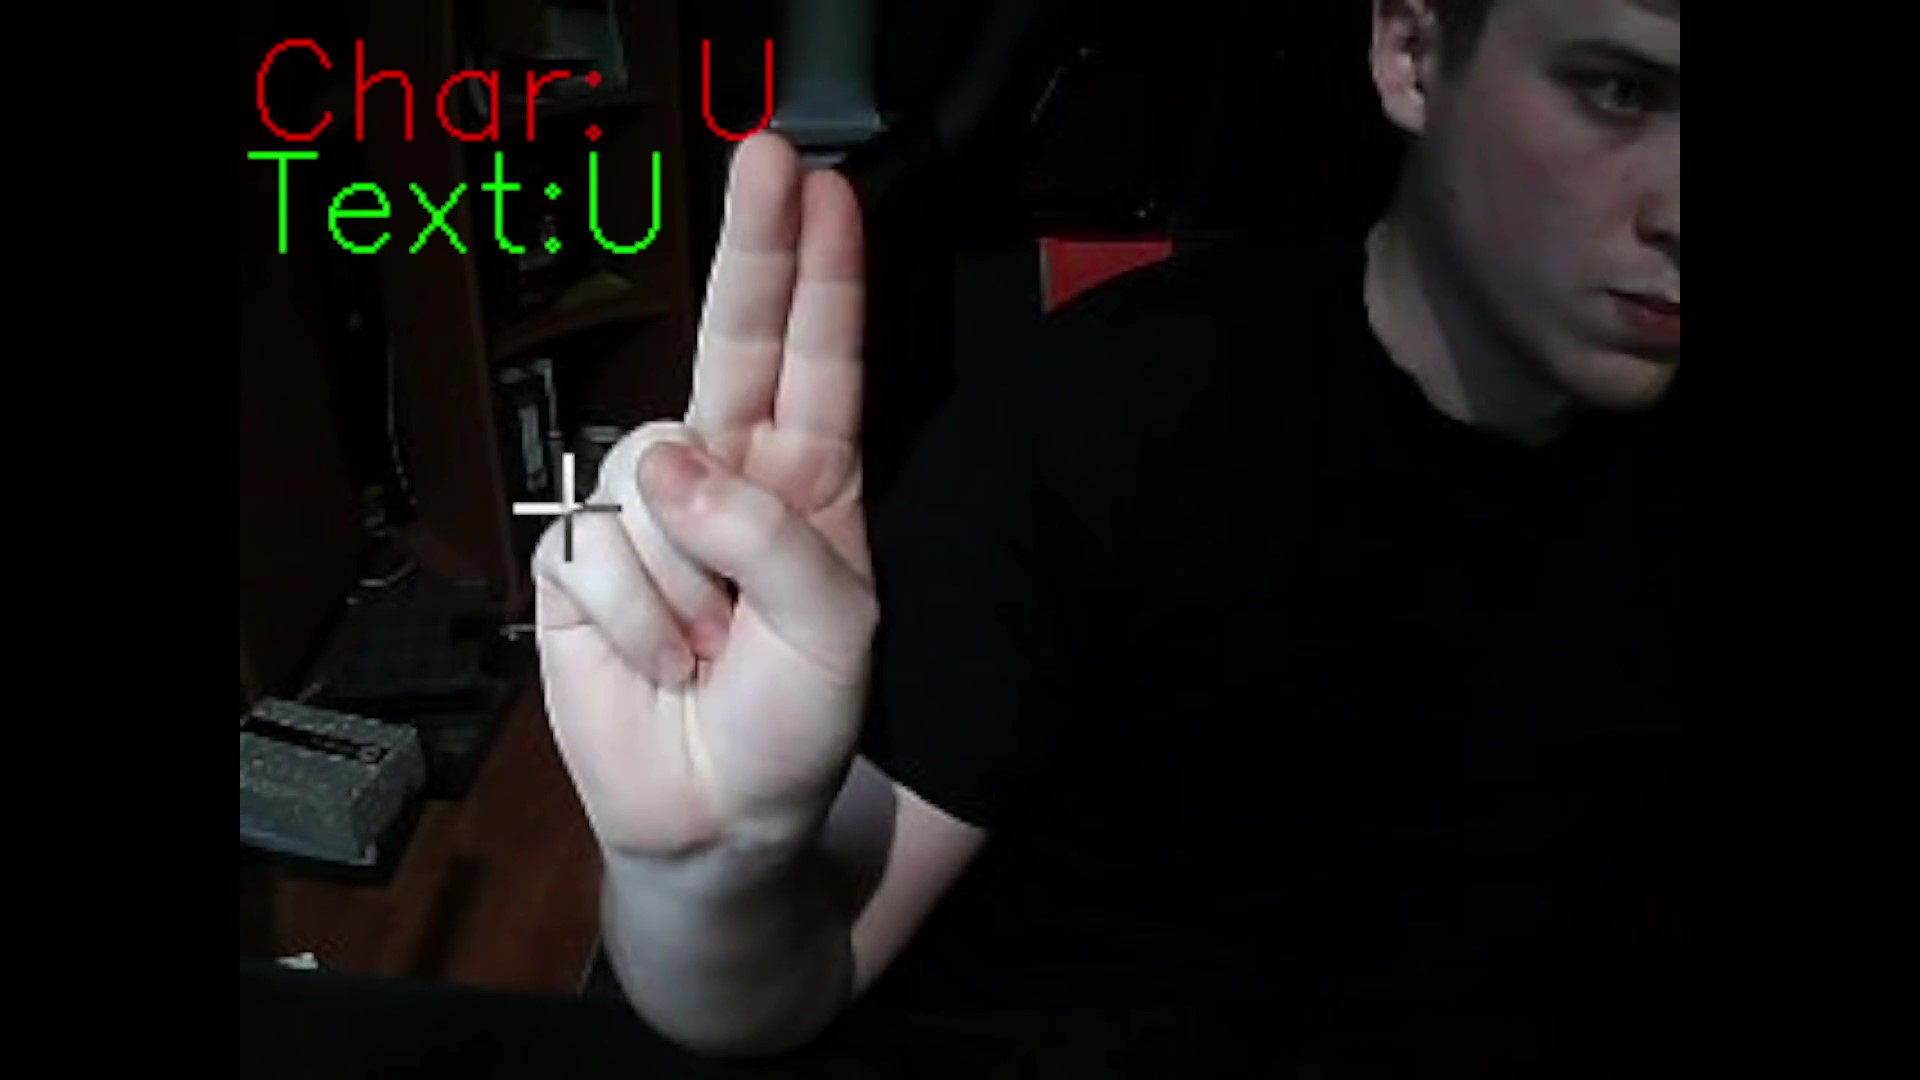
\includegraphics[scale=0.07]{U}
			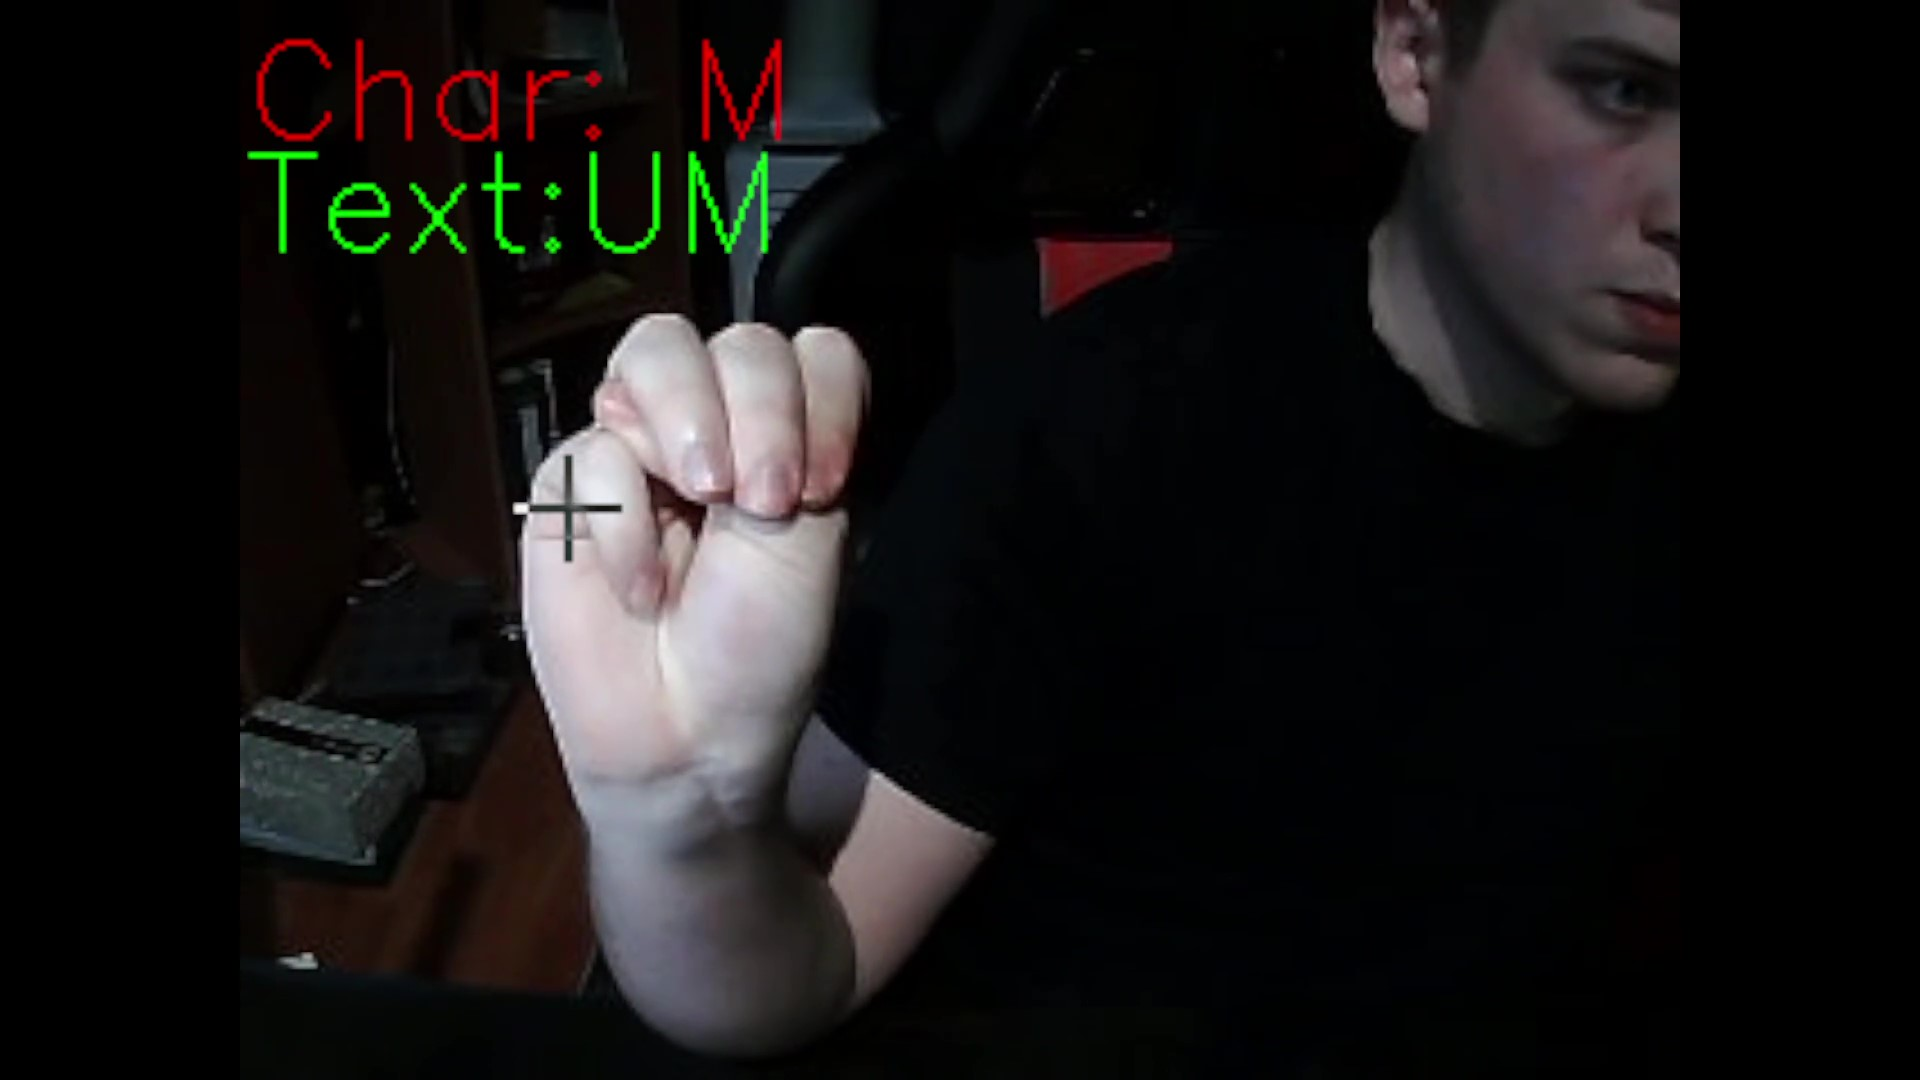
\includegraphics[scale=0.07]{M}
			
			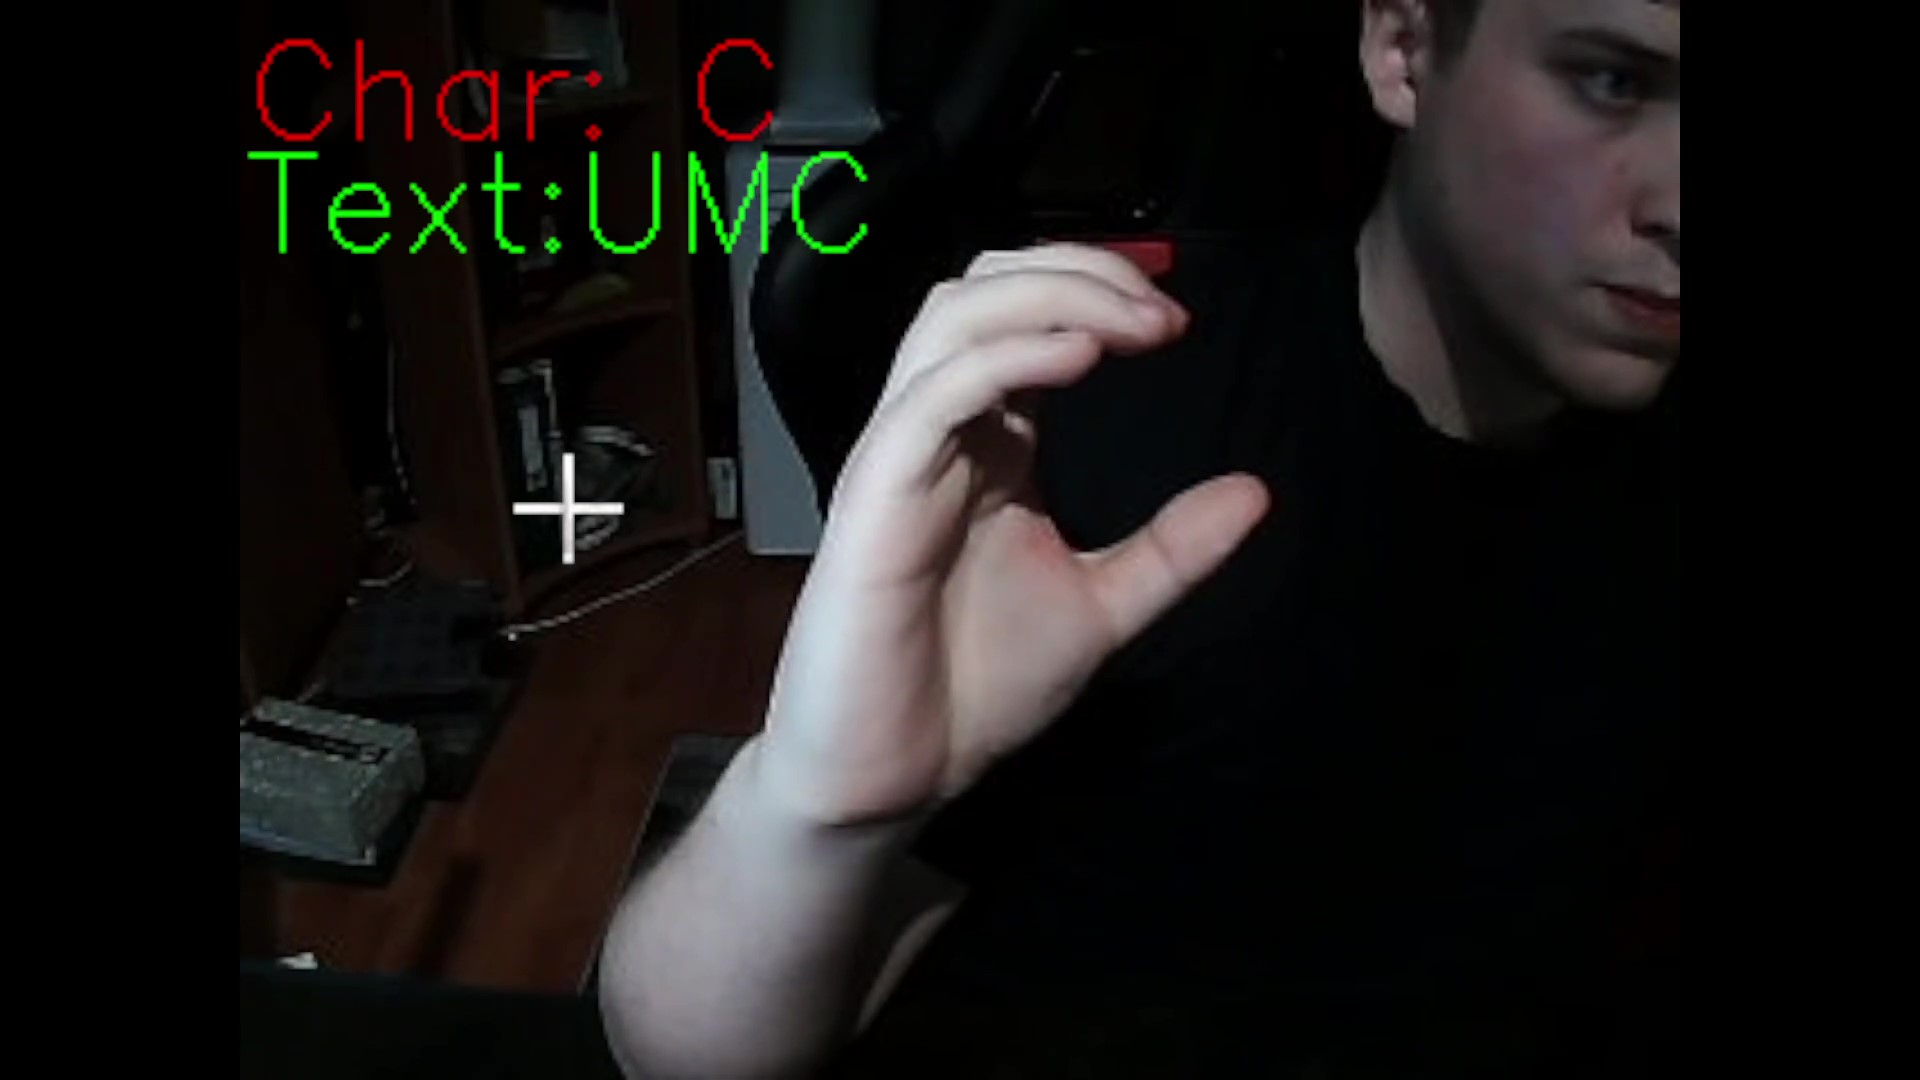
\includegraphics[scale=0.07]{C}
			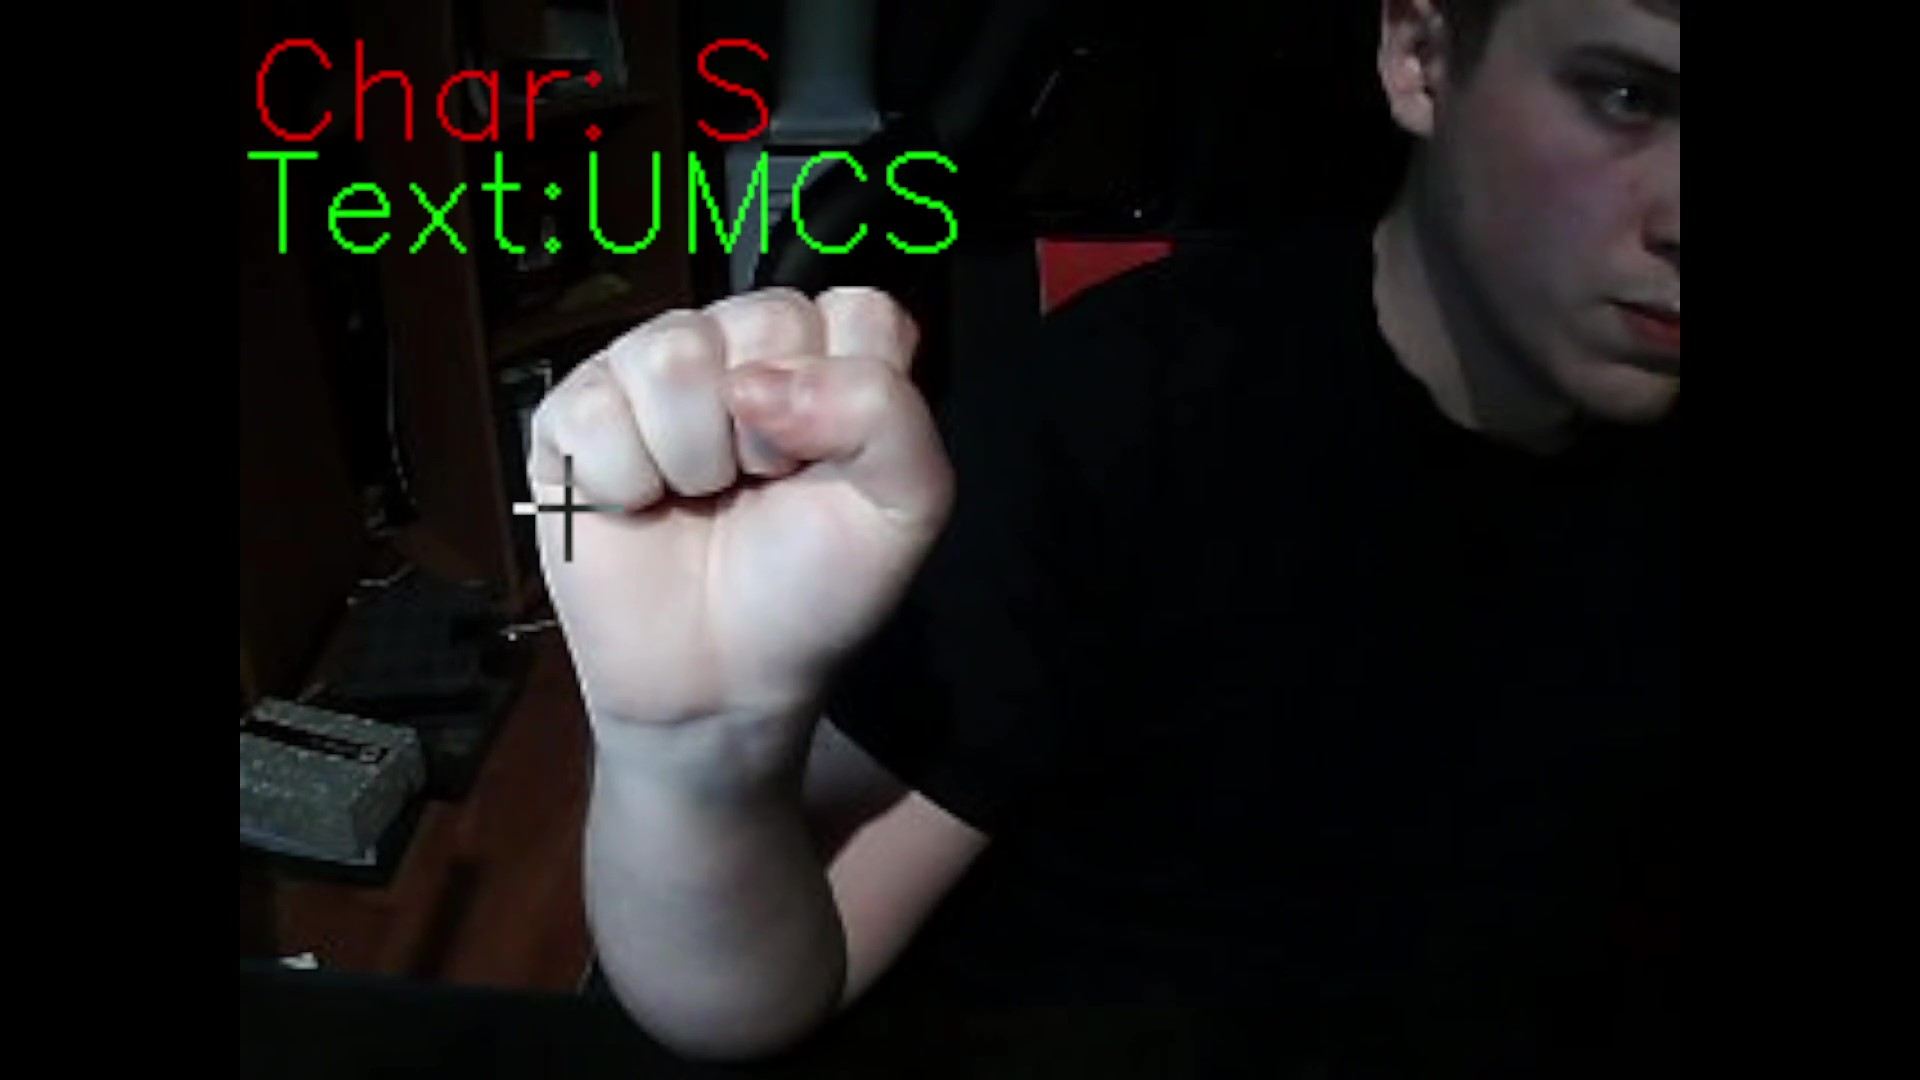
\includegraphics[scale=0.07]{S}
		\end{center}
	\end{frame}

	% Literatura
	\begin{frame}
		\frametitle{Literatura}
		\section{Literatura}
		\printbibliography
	\end{frame}

\end{document}